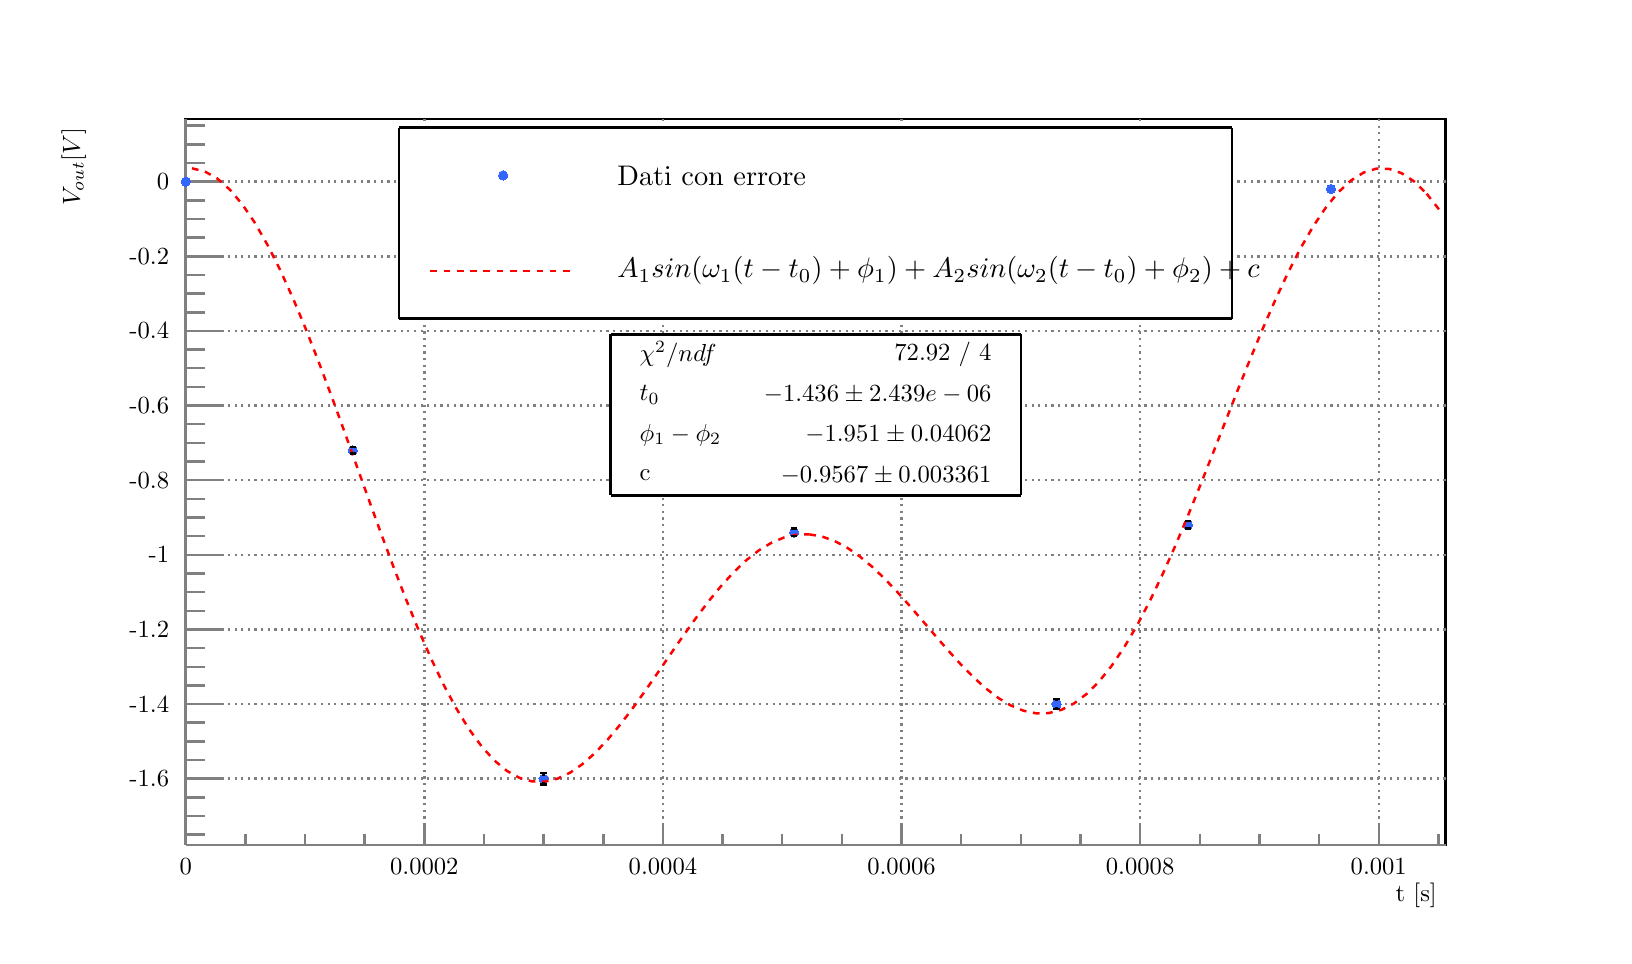
\begin{tikzpicture}
\pgfdeclareplotmark{cross} {
\pgfpathmoveto{\pgfpoint{-0.3\pgfplotmarksize}{\pgfplotmarksize}}
\pgfpathlineto{\pgfpoint{+0.3\pgfplotmarksize}{\pgfplotmarksize}}
\pgfpathlineto{\pgfpoint{+0.3\pgfplotmarksize}{0.3\pgfplotmarksize}}
\pgfpathlineto{\pgfpoint{+1\pgfplotmarksize}{0.3\pgfplotmarksize}}
\pgfpathlineto{\pgfpoint{+1\pgfplotmarksize}{-0.3\pgfplotmarksize}}
\pgfpathlineto{\pgfpoint{+0.3\pgfplotmarksize}{-0.3\pgfplotmarksize}}
\pgfpathlineto{\pgfpoint{+0.3\pgfplotmarksize}{-1.\pgfplotmarksize}}
\pgfpathlineto{\pgfpoint{-0.3\pgfplotmarksize}{-1.\pgfplotmarksize}}
\pgfpathlineto{\pgfpoint{-0.3\pgfplotmarksize}{-0.3\pgfplotmarksize}}
\pgfpathlineto{\pgfpoint{-1.\pgfplotmarksize}{-0.3\pgfplotmarksize}}
\pgfpathlineto{\pgfpoint{-1.\pgfplotmarksize}{0.3\pgfplotmarksize}}
\pgfpathlineto{\pgfpoint{-0.3\pgfplotmarksize}{0.3\pgfplotmarksize}}
\pgfpathclose
\pgfusepathqstroke
}
\pgfdeclareplotmark{cross*} {
\pgfpathmoveto{\pgfpoint{-0.3\pgfplotmarksize}{\pgfplotmarksize}}
\pgfpathlineto{\pgfpoint{+0.3\pgfplotmarksize}{\pgfplotmarksize}}
\pgfpathlineto{\pgfpoint{+0.3\pgfplotmarksize}{0.3\pgfplotmarksize}}
\pgfpathlineto{\pgfpoint{+1\pgfplotmarksize}{0.3\pgfplotmarksize}}
\pgfpathlineto{\pgfpoint{+1\pgfplotmarksize}{-0.3\pgfplotmarksize}}
\pgfpathlineto{\pgfpoint{+0.3\pgfplotmarksize}{-0.3\pgfplotmarksize}}
\pgfpathlineto{\pgfpoint{+0.3\pgfplotmarksize}{-1.\pgfplotmarksize}}
\pgfpathlineto{\pgfpoint{-0.3\pgfplotmarksize}{-1.\pgfplotmarksize}}
\pgfpathlineto{\pgfpoint{-0.3\pgfplotmarksize}{-0.3\pgfplotmarksize}}
\pgfpathlineto{\pgfpoint{-1.\pgfplotmarksize}{-0.3\pgfplotmarksize}}
\pgfpathlineto{\pgfpoint{-1.\pgfplotmarksize}{0.3\pgfplotmarksize}}
\pgfpathlineto{\pgfpoint{-0.3\pgfplotmarksize}{0.3\pgfplotmarksize}}
\pgfpathclose
\pgfusepathqfillstroke
}
\pgfdeclareplotmark{newstar} {
\pgfpathmoveto{\pgfqpoint{0pt}{\pgfplotmarksize}}
\pgfpathlineto{\pgfqpointpolar{44}{0.5\pgfplotmarksize}}
\pgfpathlineto{\pgfqpointpolar{18}{\pgfplotmarksize}}
\pgfpathlineto{\pgfqpointpolar{-20}{0.5\pgfplotmarksize}}
\pgfpathlineto{\pgfqpointpolar{-54}{\pgfplotmarksize}}
\pgfpathlineto{\pgfqpointpolar{-90}{0.5\pgfplotmarksize}}
\pgfpathlineto{\pgfqpointpolar{234}{\pgfplotmarksize}}
\pgfpathlineto{\pgfqpointpolar{198}{0.5\pgfplotmarksize}}
\pgfpathlineto{\pgfqpointpolar{162}{\pgfplotmarksize}}
\pgfpathlineto{\pgfqpointpolar{134}{0.5\pgfplotmarksize}}
\pgfpathclose
\pgfusepathqstroke
}
\pgfdeclareplotmark{newstar*} {
\pgfpathmoveto{\pgfqpoint{0pt}{\pgfplotmarksize}}
\pgfpathlineto{\pgfqpointpolar{44}{0.5\pgfplotmarksize}}
\pgfpathlineto{\pgfqpointpolar{18}{\pgfplotmarksize}}
\pgfpathlineto{\pgfqpointpolar{-20}{0.5\pgfplotmarksize}}
\pgfpathlineto{\pgfqpointpolar{-54}{\pgfplotmarksize}}
\pgfpathlineto{\pgfqpointpolar{-90}{0.5\pgfplotmarksize}}
\pgfpathlineto{\pgfqpointpolar{234}{\pgfplotmarksize}}
\pgfpathlineto{\pgfqpointpolar{198}{0.5\pgfplotmarksize}}
\pgfpathlineto{\pgfqpointpolar{162}{\pgfplotmarksize}}
\pgfpathlineto{\pgfqpointpolar{134}{0.5\pgfplotmarksize}}
\pgfpathclose
\pgfusepathqfillstroke
}
\definecolor{c}{rgb}{1,1,1};
\draw [color=c, fill=c] (0,0) rectangle (20,11.523);
\draw [color=c, fill=c] (2,1.1523) rectangle (18,10.3707);
\definecolor{c}{rgb}{0,0,0};
\draw [c,line width=0.9] (2,1.1523) -- (2,10.3707) -- (18,10.3707) -- (18,1.1523) -- (2,1.1523);
\definecolor{c}{rgb}{1,1,1};
\draw [color=c, fill=c] (2,1.1523) rectangle (18,10.3707);
\definecolor{c}{rgb}{0,0,0};
\draw [c,line width=0.9] (2,1.1523) -- (2,10.3707) -- (18,10.3707) -- (18,1.1523) -- (2,1.1523);
\definecolor{c}{rgb}{0.5,0.5,0.5};
\draw [c,line width=0.9] (2,1.1523) -- (18,1.1523);
\draw [c,dash pattern=on 0.80pt off 1.60pt ,line width=0.9] (2,10.3707) -- (2,1.1523);
\draw [c,dash pattern=on 0.80pt off 1.60pt ,line width=0.9] (5.0303,10.3707) -- (5.0303,1.1523);
\draw [c,dash pattern=on 0.80pt off 1.60pt ,line width=0.9] (8.06061,10.3707) -- (8.06061,1.1523);
\draw [c,dash pattern=on 0.80pt off 1.60pt ,line width=0.9] (11.0909,10.3707) -- (11.0909,1.1523);
\draw [c,dash pattern=on 0.80pt off 1.60pt ,line width=0.9] (14.1212,10.3707) -- (14.1212,1.1523);
\draw [c,dash pattern=on 0.80pt off 1.60pt ,line width=0.9] (17.1515,10.3707) -- (17.1515,1.1523);
\draw [c,dash pattern=on 0.80pt off 1.60pt ,line width=0.9] (17.1515,10.3707) -- (17.1515,1.1523);
\draw [c,line width=0.9] (2,1.1523) -- (2,10.3707);
\draw [c,dash pattern=on 0.80pt off 1.60pt ,line width=0.9] (18,1.99206) -- (2,1.99206);
\draw [c,dash pattern=on 0.80pt off 1.60pt ,line width=0.9] (18,2.93982) -- (2,2.93982);
\draw [c,dash pattern=on 0.80pt off 1.60pt ,line width=0.9] (18,3.88757) -- (2,3.88757);
\draw [c,dash pattern=on 0.80pt off 1.60pt ,line width=0.9] (18,4.83533) -- (2,4.83533);
\draw [c,dash pattern=on 0.80pt off 1.60pt ,line width=0.9] (18,5.78308) -- (2,5.78308);
\draw [c,dash pattern=on 0.80pt off 1.60pt ,line width=0.9] (18,6.73084) -- (2,6.73084);
\draw [c,dash pattern=on 0.80pt off 1.60pt ,line width=0.9] (18,7.6786) -- (2,7.6786);
\draw [c,dash pattern=on 0.80pt off 1.60pt ,line width=0.9] (18,8.62635) -- (2,8.62635);
\draw [c,dash pattern=on 0.80pt off 1.60pt ,line width=0.9] (18,9.57411) -- (2,9.57411);
\draw [c,dash pattern=on 0.80pt off 1.60pt ,line width=0.9] (18,1.99206) -- (2,1.99206);
\draw [c,dash pattern=on 0.80pt off 1.60pt ,line width=0.9] (18,9.57411) -- (2,9.57411);
\draw [c,line width=0.9] (2,1.1523) -- (18,1.1523);
\draw [c,line width=0.9] (2,1.42886) -- (2,1.1523);
\draw [c,line width=0.9] (2.75758,1.29058) -- (2.75758,1.1523);
\draw [c,line width=0.9] (3.51515,1.29058) -- (3.51515,1.1523);
\draw [c,line width=0.9] (4.27273,1.29058) -- (4.27273,1.1523);
\draw [c,line width=0.9] (5.0303,1.42886) -- (5.0303,1.1523);
\draw [c,line width=0.9] (5.78788,1.29058) -- (5.78788,1.1523);
\draw [c,line width=0.9] (6.54545,1.29058) -- (6.54545,1.1523);
\draw [c,line width=0.9] (7.30303,1.29058) -- (7.30303,1.1523);
\draw [c,line width=0.9] (8.06061,1.42886) -- (8.06061,1.1523);
\draw [c,line width=0.9] (8.81818,1.29058) -- (8.81818,1.1523);
\draw [c,line width=0.9] (9.57576,1.29058) -- (9.57576,1.1523);
\draw [c,line width=0.9] (10.3333,1.29058) -- (10.3333,1.1523);
\draw [c,line width=0.9] (11.0909,1.42886) -- (11.0909,1.1523);
\draw [c,line width=0.9] (11.8485,1.29058) -- (11.8485,1.1523);
\draw [c,line width=0.9] (12.6061,1.29058) -- (12.6061,1.1523);
\draw [c,line width=0.9] (13.3636,1.29058) -- (13.3636,1.1523);
\draw [c,line width=0.9] (14.1212,1.42886) -- (14.1212,1.1523);
\draw [c,line width=0.9] (14.8788,1.29058) -- (14.8788,1.1523);
\draw [c,line width=0.9] (15.6364,1.29058) -- (15.6364,1.1523);
\draw [c,line width=0.9] (16.3939,1.29058) -- (16.3939,1.1523);
\draw [c,line width=0.9] (17.1515,1.42886) -- (17.1515,1.1523);
\draw [c,line width=0.9] (17.1515,1.42886) -- (17.1515,1.1523);
\draw [c,line width=0.9] (17.9091,1.29058) -- (17.9091,1.1523);
\definecolor{c}{rgb}{0,0,0};
\draw [anchor=base] (2,0.772044) node[scale=0.890168, color=c, rotate=0]{0};
\draw [anchor=base] (5.0303,0.772044) node[scale=0.890168, color=c, rotate=0]{0.0002};
\draw [anchor=base] (8.06061,0.772044) node[scale=0.890168, color=c, rotate=0]{0.0004};
\draw [anchor=base] (11.0909,0.772044) node[scale=0.890168, color=c, rotate=0]{0.0006};
\draw [anchor=base] (14.1212,0.772044) node[scale=0.890168, color=c, rotate=0]{0.0008};
\draw [anchor=base] (17.1515,0.772044) node[scale=0.890168, color=c, rotate=0]{0.001};
\draw [anchor= east] (18,0.507014) node[scale=0.890168, color=c, rotate=0]{t [s]};
\definecolor{c}{rgb}{0.5,0.5,0.5};
\draw [c,line width=0.9] (2,1.1523) -- (2,10.3707);
\draw [c,line width=0.9] (2.48,1.99206) -- (2,1.99206);
\draw [c,line width=0.9] (2.24,2.229) -- (2,2.229);
\draw [c,line width=0.9] (2.24,2.46594) -- (2,2.46594);
\draw [c,line width=0.9] (2.24,2.70288) -- (2,2.70288);
\draw [c,line width=0.9] (2.48,2.93982) -- (2,2.93982);
\draw [c,line width=0.9] (2.24,3.17676) -- (2,3.17676);
\draw [c,line width=0.9] (2.24,3.4137) -- (2,3.4137);
\draw [c,line width=0.9] (2.24,3.65063) -- (2,3.65063);
\draw [c,line width=0.9] (2.48,3.88757) -- (2,3.88757);
\draw [c,line width=0.9] (2.24,4.12451) -- (2,4.12451);
\draw [c,line width=0.9] (2.24,4.36145) -- (2,4.36145);
\draw [c,line width=0.9] (2.24,4.59839) -- (2,4.59839);
\draw [c,line width=0.9] (2.48,4.83533) -- (2,4.83533);
\draw [c,line width=0.9] (2.24,5.07227) -- (2,5.07227);
\draw [c,line width=0.9] (2.24,5.30921) -- (2,5.30921);
\draw [c,line width=0.9] (2.24,5.54614) -- (2,5.54614);
\draw [c,line width=0.9] (2.48,5.78308) -- (2,5.78308);
\draw [c,line width=0.9] (2.24,6.02002) -- (2,6.02002);
\draw [c,line width=0.9] (2.24,6.25696) -- (2,6.25696);
\draw [c,line width=0.9] (2.24,6.4939) -- (2,6.4939);
\draw [c,line width=0.9] (2.48,6.73084) -- (2,6.73084);
\draw [c,line width=0.9] (2.24,6.96778) -- (2,6.96778);
\draw [c,line width=0.9] (2.24,7.20472) -- (2,7.20472);
\draw [c,line width=0.9] (2.24,7.44166) -- (2,7.44166);
\draw [c,line width=0.9] (2.48,7.6786) -- (2,7.6786);
\draw [c,line width=0.9] (2.24,7.91553) -- (2,7.91553);
\draw [c,line width=0.9] (2.24,8.15247) -- (2,8.15247);
\draw [c,line width=0.9] (2.24,8.38941) -- (2,8.38941);
\draw [c,line width=0.9] (2.48,8.62635) -- (2,8.62635);
\draw [c,line width=0.9] (2.24,8.86329) -- (2,8.86329);
\draw [c,line width=0.9] (2.24,9.10023) -- (2,9.10023);
\draw [c,line width=0.9] (2.24,9.33717) -- (2,9.33717);
\draw [c,line width=0.9] (2.48,9.57411) -- (2,9.57411);
\draw [c,line width=0.9] (2.48,1.99206) -- (2,1.99206);
\draw [c,line width=0.9] (2.24,1.75512) -- (2,1.75512);
\draw [c,line width=0.9] (2.24,1.51818) -- (2,1.51818);
\draw [c,line width=0.9] (2.24,1.28125) -- (2,1.28125);
\draw [c,line width=0.9] (2.48,9.57411) -- (2,9.57411);
\draw [c,line width=0.9] (2.24,9.81104) -- (2,9.81104);
\draw [c,line width=0.9] (2.24,10.048) -- (2,10.048);
\draw [c,line width=0.9] (2.24,10.2849) -- (2,10.2849);
\definecolor{c}{rgb}{0,0,0};
\draw [anchor= east] (1.9,1.99206) node[scale=0.890168, color=c, rotate=0]{-1.6};
\draw [anchor= east] (1.9,2.93982) node[scale=0.890168, color=c, rotate=0]{-1.4};
\draw [anchor= east] (1.9,3.88757) node[scale=0.890168, color=c, rotate=0]{-1.2};
\draw [anchor= east] (1.9,4.83533) node[scale=0.890168, color=c, rotate=0]{-1};
\draw [anchor= east] (1.9,5.78308) node[scale=0.890168, color=c, rotate=0]{-0.8};
\draw [anchor= east] (1.9,6.73084) node[scale=0.890168, color=c, rotate=0]{-0.6};
\draw [anchor= east] (1.9,7.6786) node[scale=0.890168, color=c, rotate=0]{-0.4};
\draw [anchor= east] (1.9,8.62635) node[scale=0.890168, color=c, rotate=0]{-0.2};
\draw [anchor= east] (1.9,9.57411) node[scale=0.890168, color=c, rotate=0]{0};
\draw [anchor= east] (0.578557,10.3707) node[scale=0.890168, color=c, rotate=90]{$V_{out} [V]$};
\definecolor{c}{rgb}{0.2,0.4,1};
\foreach \P in {(2,9.57411), (4.12121,6.16219), (6.54545,1.99206), (9.72727,5.11966), (13.0606,2.93982), (14.7273,5.21443), (16.5455,9.47933)}{\draw[mark options={color=c,fill=c},mark size=1.681682pt, line width=0.000000pt, mark=*] plot coordinates
 {\P};}
\definecolor{c}{rgb}{1,0,0};
\draw [c,dash pattern=on 2.40pt off 2.40pt ,line width=0.9] (2.08,9.74339) -- (2.24,9.70488) -- (2.4,9.61472) -- (2.56,9.47397) -- (2.72,9.2844) -- (2.88,9.04855) -- (3.04,8.76964) -- (3.2,8.45151) -- (3.36,8.09858) -- (3.52,7.71579) --
 (3.68,7.30848) -- (3.84,6.88232) -- (4,6.44324) -- (4.16,5.99728) -- (4.32,5.55056) -- (4.48,5.10911) -- (4.64,4.67882) -- (4.8,4.26533) -- (4.96,3.87394) -- (5.12,3.50951) -- (5.28,3.17641) -- (5.44,2.87844) -- (5.6,2.61878) -- (5.76,2.3999) --
 (5.92,2.22361) -- (6.08,2.09094) -- (6.24,2.00222) -- (6.4,1.95702) -- (6.56,1.95418) -- (6.72,1.99188) -- (6.88,2.06761) -- (7.04,2.17829) -- (7.2,2.32028) -- (7.36,2.48949) -- (7.52,2.68143) -- (7.68,2.89131) -- (7.84,3.11413) -- (8,3.34477) --
 (8.16,3.57809) -- (8.32,3.80903) -- (8.48,4.03268) -- (8.64,4.24438) -- (8.8,4.43985) -- (8.96,4.61518) -- (9.12,4.76697) -- (9.28,4.89239) -- (9.44,4.98917) -- (9.6,5.05571) -- (9.76,5.09108) -- (9.92,5.09502);
\draw [c,dash pattern=on 2.40pt off 2.40pt ,line width=0.9] (9.92,5.09502) -- (10.08,5.06796) -- (10.24,5.01102) -- (10.4,4.92595) -- (10.56,4.81515) -- (10.72,4.68156) -- (10.88,4.52868) -- (11.04,4.36044) -- (11.2,4.18113) -- (11.36,3.99536) --
 (11.52,3.80796) -- (11.68,3.62383) -- (11.84,3.44794) -- (12,3.28518) -- (12.16,3.14024) -- (12.32,3.0176) -- (12.48,2.92136) -- (12.64,2.85523) -- (12.8,2.82239) -- (12.96,2.82548) -- (13.12,2.86651) -- (13.28,2.94683) -- (13.44,3.06709) --
 (13.6,3.22725) -- (13.76,3.4265) -- (13.92,3.66335) -- (14.08,3.93558) -- (14.24,4.24033) -- (14.4,4.57408) -- (14.56,4.93276) -- (14.72,5.31176) -- (14.88,5.70606) -- (15.04,6.11026) -- (15.2,6.5187) -- (15.36,6.92556) -- (15.52,7.32491) --
 (15.68,7.71085) -- (15.84,8.07762) -- (16,8.41965) -- (16.16,8.73167) -- (16.32,9.00885) -- (16.48,9.24679) -- (16.64,9.44169) -- (16.8,9.59034) -- (16.96,9.69022) -- (17.12,9.73952) -- (17.28,9.7372) -- (17.44,9.68298) -- (17.6,9.57734) --
 (17.76,9.42157);
\draw [c,dash pattern=on 2.40pt off 2.40pt ,line width=0.9] (17.76,9.42157) -- (17.92,9.21769);
\definecolor{c}{rgb}{1,1,1};
\draw [color=c, fill=c] (7.39479,5.59118) rectangle (12.6052,7.63527);
\definecolor{c}{rgb}{0,0,0};
\draw [c,line width=0.9] (7.39479,5.59118) -- (12.6052,5.59118);
\draw [c,line width=0.9] (12.6052,5.59118) -- (12.6052,7.63527);
\draw [c,line width=0.9] (12.6052,7.63527) -- (7.39479,7.63527);
\draw [c,line width=0.9] (7.39479,7.63527) -- (7.39479,5.59118);
\draw [anchor= west] (7.65531,7.37976) node[scale=0.890168, color=c, rotate=0]{$\chi^{2} / ndf $};
\draw [anchor= east] (12.3447,7.37976) node[scale=0.890168, color=c, rotate=0]{ 72.92 / 4};
\draw [anchor= west] (7.65531,6.86874) node[scale=0.890168, color=c, rotate=0]{$t_{0}    $};
\draw [anchor= east] (12.3447,6.86874) node[scale=0.890168, color=c, rotate=0]{$ -1.436 \pm 2.439e-06$};
\draw [anchor= west] (7.65531,6.35772) node[scale=0.890168, color=c, rotate=0]{$\phi_{1} - \phi_{2} $};
\draw [anchor= east] (12.3447,6.35772) node[scale=0.890168, color=c, rotate=0]{$ -1.951 \pm 0.04062$};
\draw [anchor= west] (7.65531,5.84669) node[scale=0.890168, color=c, rotate=0]{c        };
\draw [anchor= east] (12.3447,5.84669) node[scale=0.890168, color=c, rotate=0]{$ -0.9567 \pm 0.003361$};
\draw [c,line width=0.9] (4.12121,6.20227) -- (4.12121,6.20319);
\draw [c,line width=0.9] (4.08113,6.20319) -- (4.16129,6.20319);
\draw [c,line width=0.9] (4.12121,6.12211) -- (4.12121,6.12118);
\draw [c,line width=0.9] (4.08113,6.12118) -- (4.16129,6.12118);
\draw [c,line width=0.9] (6.54545,2.03214) -- (6.54545,2.06362);
\draw [c,line width=0.9] (6.50537,2.06362) -- (6.58553,2.06362);
\draw [c,line width=0.9] (6.54545,1.95198) -- (6.54545,1.92051);
\draw [c,line width=0.9] (6.50537,1.92051) -- (6.58553,1.92051);
\draw [c,line width=0.9] (9.72727,5.15974) -- (9.72727,5.16758);
\draw [c,line width=0.9] (9.68719,5.16758) -- (9.76735,5.16758);
\draw [c,line width=0.9] (9.72727,5.07958) -- (9.72727,5.07173);
\draw [c,line width=0.9] (9.68719,5.07173) -- (9.76735,5.07173);
\draw [c,line width=0.9] (13.0606,2.9799) -- (13.0606,3.00392);
\draw [c,line width=0.9] (13.0205,3.00392) -- (13.1007,3.00392);
\draw [c,line width=0.9] (13.0606,2.89974) -- (13.0606,2.87571);
\draw [c,line width=0.9] (13.0205,2.87571) -- (13.1007,2.87571);
\draw [c,line width=0.9] (14.7273,5.25451) -- (14.7273,5.26169);
\draw [c,line width=0.9] (14.6872,5.26169) -- (14.7674,5.26169);
\draw [c,line width=0.9] (14.7273,5.17435) -- (14.7273,5.16717);
\draw [c,line width=0.9] (14.6872,5.16717) -- (14.7674,5.16717);
\definecolor{c}{rgb}{1,1,1};
\draw [color=c, fill=c] (7.39479,5.59118) rectangle (12.6052,7.63527);
\definecolor{c}{rgb}{0,0,0};
\draw [c,line width=0.9] (7.39479,5.59118) -- (12.6052,5.59118);
\draw [c,line width=0.9] (12.6052,5.59118) -- (12.6052,7.63527);
\draw [c,line width=0.9] (12.6052,7.63527) -- (7.39479,7.63527);
\draw [c,line width=0.9] (7.39479,7.63527) -- (7.39479,5.59118);
\draw [anchor= west] (7.65531,7.37976) node[scale=0.890168, color=c, rotate=0]{$\chi^{2} / ndf $};
\draw [anchor= east] (12.3447,7.37976) node[scale=0.890168, color=c, rotate=0]{ 72.92 / 4};
\draw [anchor= west] (7.65531,6.86874) node[scale=0.890168, color=c, rotate=0]{$t_{0}    $};
\draw [anchor= east] (12.3447,6.86874) node[scale=0.890168, color=c, rotate=0]{$ -1.436 \pm 2.439e-06$};
\draw [anchor= west] (7.65531,6.35772) node[scale=0.890168, color=c, rotate=0]{$\phi_{1} - \phi_{2} $};
\draw [anchor= east] (12.3447,6.35772) node[scale=0.890168, color=c, rotate=0]{$ -1.951 \pm 0.04062$};
\draw [anchor= west] (7.65531,5.84669) node[scale=0.890168, color=c, rotate=0]{c        };
\draw [anchor= east] (12.3447,5.84669) node[scale=0.890168, color=c, rotate=0]{$ -0.9567 \pm 0.003361$};
\definecolor{c}{rgb}{1,1,1};
\draw [color=c, fill=c] (4.70942,7.83567) rectangle (15.2906,10.2605);
\definecolor{c}{rgb}{0,0,0};
\draw [c,line width=0.9] (4.70942,7.83567) -- (15.2906,7.83567);
\draw [c,line width=0.9] (15.2906,7.83567) -- (15.2906,10.2605);
\draw [c,line width=0.9] (15.2906,10.2605) -- (4.70942,10.2605);
\draw [c,line width=0.9] (4.70942,10.2605) -- (4.70942,7.83567);
\draw [anchor= west] (7.35471,9.65431) node[scale=1.02369, color=c, rotate=0]{Dati con errore};
\definecolor{c}{rgb}{0.2,0.4,1};
\foreach \P in {(6.03206,9.65431)}{\draw[mark options={color=c,fill=c},mark size=1.681682pt, line width=0.000000pt, mark=*] plot coordinates {\P};}
\definecolor{c}{rgb}{0,0,0};
\draw [anchor= west] (7.35471,8.44188) node[scale=1.02369, color=c, rotate=0]{$A_{1}sin(\omega_{1} (t-t_{0}) + \phi_{1})+A_{2}sin(\omega_{2} (t-t_{0}) + \phi_{2}) + c$};
\definecolor{c}{rgb}{1,0,0};
\draw [c,dash pattern=on 2.40pt off 2.40pt ,line width=0.9] (5.10621,8.44188) -- (6.95792,8.44188);
\end{tikzpicture}
